% Standalone block scheme for the gantry augmentation (iterate on this figure alone).
% Style: Hoekstra et al. (2025) Fig. 1. Routing shown with wires, detail in the formulas.
% Compile: pdflatex jan-blockscheme.tex
\documentclass[border=10pt]{standalone}
\usepackage{tikz}
\usetikzlibrary{arrows.meta, calc}
\usepackage{amsmath}

\begin{document}
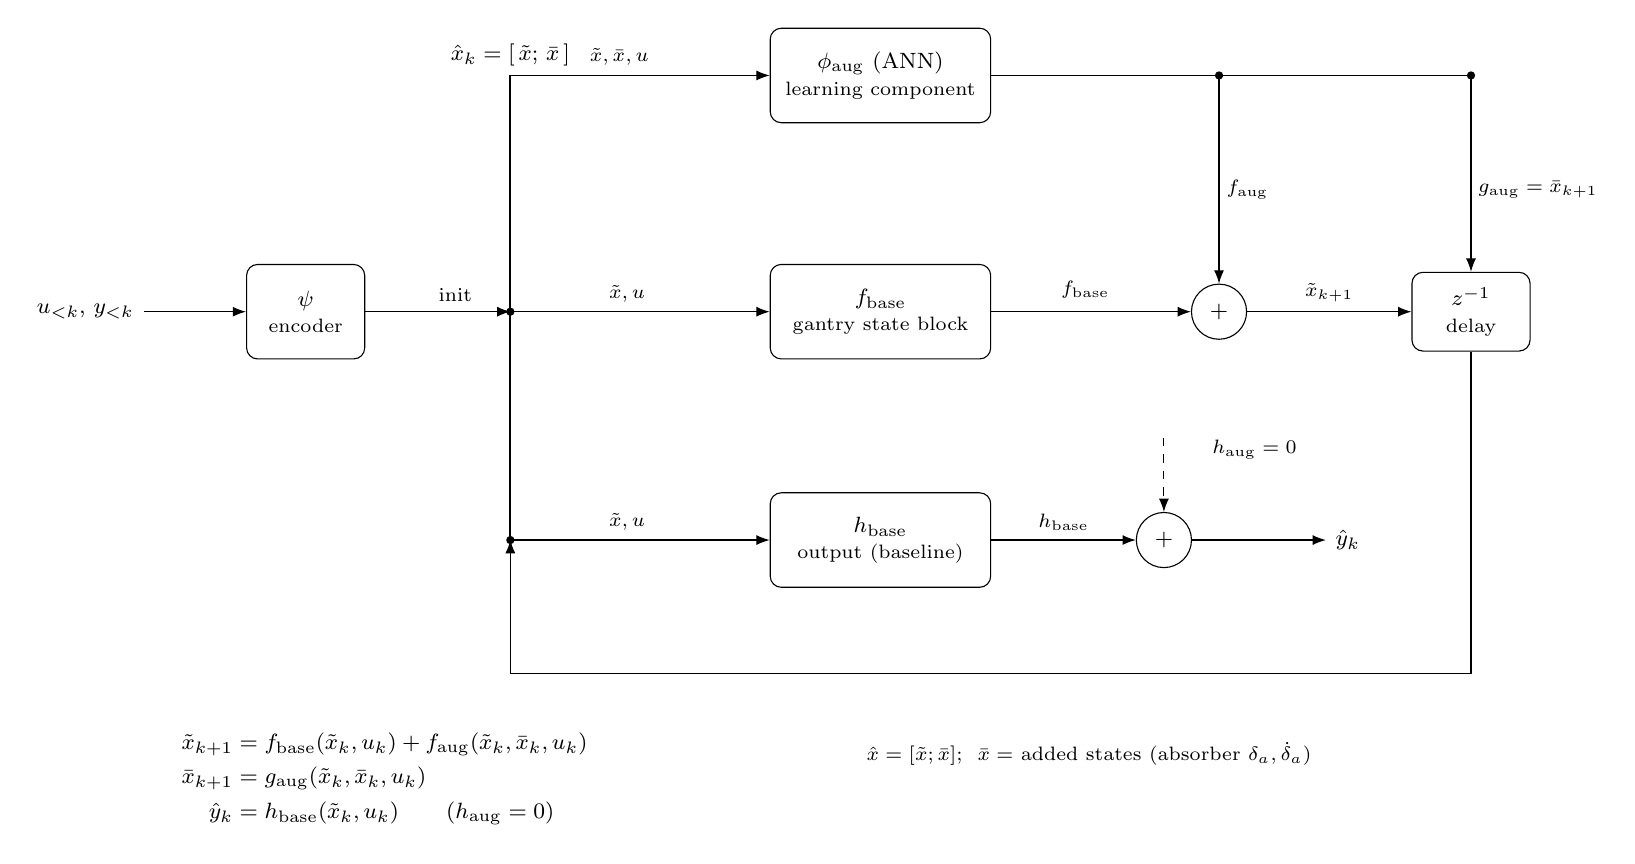
\begin{tikzpicture}[>=Latex, font=\footnotesize,
  block/.style={draw, rounded corners, minimum width=28mm, minimum height=12mm, align=center},
  small/.style={draw, rounded corners, minimum width=15mm, minimum height=10mm, align=center},
  sum/.style={draw, circle, minimum size=7mm, inner sep=0pt},
  jn/.style={circle, fill, minimum size=3pt, inner sep=0pt}]

% ---------- blocks ----------
\node[block] (ann)   at (0, 3.0)   {$\phi_{\mathrm{aug}}$ (ANN)\\{\scriptsize learning component}};
\node[block] (fbase) at (0, 0)     {$f_{\mathrm{base}}$\\{\scriptsize gantry state block}};
\node[block] (hbase) at (0,-2.9)   {$h_{\mathrm{base}}$\\{\scriptsize output (baseline)}};

% ---------- encoder ----------
\node[block, minimum width=15mm] (enc) at (-7.3,0) {$\psi$\\{\scriptsize encoder}};
\draw[<-] (enc.west) -- ++(-1.3,0) node[left]{$u_{<k},\,y_{<k}$};

% ---------- state bus  x_hat_k = [xtilde ; xbar] ----------
\draw[thick] (-4.7,-2.9) -- (-4.7,3.0);
\node[above] at (-4.7,3.0) {$\hat{x}_k=[\,\tilde{x};\,\bar{x}\,]$};
\draw[->] (enc.east) -- (-4.7,0) node[pos=0.62,above]{\scriptsize init};

% taps (u bundled into the label; no separate u wire)
\draw[->] (-4.7, 3.0) -- (ann.west)   node[pos=0.42,above]{\scriptsize $\tilde{x},\bar{x},u$};
\draw[->] (-4.7, 0.0) -- (fbase.west) node[pos=0.45,above]{\scriptsize $\tilde{x},u$};
\draw[->] (-4.7,-2.9) -- (hbase.west) node[pos=0.45,above]{\scriptsize $\tilde{x},u$};
\node[jn] at (-4.7,0.0) {};

% ---------- xtilde update (f_base + f_aug, summed) and xbar update (g_aug, bypasses) ----------
% f_aug is added to f_base (Theta states have a baseline);
% g_aug bypasses the sum (added states have no baseline) and goes straight to the delay.
\node[sum] (sum) at (4.3,0) {$+$};
\draw[->] (fbase.east) -- (sum.west);
\node at (2.6,0.28) {\scriptsize $f_{\mathrm{base}}$};

\node[small] (delay) at (7.5,0) {$z^{-1}$\\{\scriptsize delay}};
\draw[->] (sum.east) -- (delay.west) node[pos=0.5,above]{\scriptsize $\tilde{x}_{k+1}$};

% ANN rail across the top: f_aug drops into the sum, g_aug drops straight into the delay
\draw[-] (ann.east) -- (7.5,3.0);
\node[jn] at (4.3,3.0) {};
\node[jn] at (7.5,3.0) {};
\draw[->] (4.3,3.0) -- (sum.north);
\draw[->] (7.5,3.0) -- (delay.north);
\node at (4.66,1.55) {\scriptsize $f_{\mathrm{aug}}$};
\node at (8.35,1.55) {\scriptsize $g_{\mathrm{aug}}=\bar{x}_{k+1}$};

% feedback: delayed full state back onto the state bus
\draw[->] (delay.south) -- (7.5,-4.6) -| (-4.7,-2.9);
\node[jn] at (-4.7,-2.9) {};

% ---------- output readout: yhat = h_base (+) h_aug, h_aug = 0 ----------
\node[sum] (osum) at (3.6,-2.9) {$+$};
\draw[->] (hbase.east) -- (osum.west) node[pos=0.5,above]{\scriptsize $h_{\mathrm{base}}$};
\draw[->, dashed] (3.6,-1.6) -- (osum.north);
\node at (4.75,-1.75) {\scriptsize $h_{\mathrm{aug}}=0$};
\draw[->] (osum.east) -- ++(1.7,0) node[right]{$\hat{y}_k$};

% ---------- equation legend under the diagram ----------
\node[anchor=north west, align=left] at (-9.0,-5.2) {%
  $\begin{aligned}
    \tilde{x}_{k+1} &= f_{\mathrm{base}}(\tilde{x}_k,u_k) + f_{\mathrm{aug}}(\tilde{x}_k,\bar{x}_k,u_k)\\
    \bar{x}_{k+1}    &= g_{\mathrm{aug}}(\tilde{x}_k,\bar{x}_k,u_k)\\
    \hat{y}_k        &= h_{\mathrm{base}}(\tilde{x}_k,u_k) \qquad (h_{\mathrm{aug}}=0)
  \end{aligned}$};
\node[anchor=north west, align=left] at (-0.3,-5.35) {%
  {\scriptsize $\hat{x}=[\tilde{x};\bar{x}]$;\ \ $\bar{x}=$ added states (absorber $\delta_a,\dot\delta_a$)}};

\end{tikzpicture}
\end{document}
